% =============================================================================
%  portopt : documentation méthodologique
%  Compilation : cd docs && latexmk -xelatex methodology.tex
% =============================================================================
\documentclass[11pt,a4paper]{article}

% ----------------------------------------------------------------- langue, polices
\usepackage{polyglossia}
\setdefaultlanguage{french}
\usepackage{amsmath,amssymb,amsthm,mathtools}
\usepackage[math-style=ISO,bold-style=ISO]{unicode-math}
\setmainfont{Latin Modern Roman}[SmallCapsFont={Latin Modern Roman Caps}]
\setmathfont{Latin Modern Math}
\setsansfont{space-grotesk-400.ttf}[
  Path=../portopt/fonts/, BoldFont=space-grotesk-600.ttf, Scale=0.95,
  SmallCapsFont=space-grotesk-400.ttf, BoldFeatures={SmallCapsFont=space-grotesk-600.ttf}]
\setmonofont{space-mono-400.ttf}[Path=../portopt/fonts/, Scale=0.86]
\newfontfamily\headfont{space-grotesk-600.ttf}[Path=../portopt/fonts/]
\usepackage[autostyle]{csquotes}

% ----------------------------------------------------------------- mise en page
\usepackage[a4paper,margin=2.5cm,headheight=14pt]{geometry}
\usepackage{microtype}
\usepackage{xcolor}
\definecolor{accent}{HTML}{2A78D6}
\definecolor{accentsoft}{HTML}{F2F7FD}
\definecolor{warm}{HTML}{EB6834}
\definecolor{warmsoft}{HTML}{FDF3EE}
\definecolor{green}{HTML}{1BAF7A}
\definecolor{greensoft}{HTML}{EEFAF5}
\definecolor{ink}{HTML}{0B0B0B}
\definecolor{ink2}{HTML}{52514E}
\definecolor{rule}{HTML}{E4E3DF}

\usepackage{graphicx}
\graphicspath{{figures/}}
\usepackage[font=small,labelfont={sf,bf},labelsep=period,skip=6pt]{caption}
\usepackage{booktabs,tabularx,array}
\usepackage[section]{placeins}
\usepackage{enumitem}
\setlist{itemsep=2pt,topsep=4pt,leftmargin=*}
\usepackage{fancyhdr}
\usepackage{titlesec}
\usepackage[most]{tcolorbox}
\usepackage{listings}
\usepackage{tikz}
\usetikzlibrary{positioning,arrows.meta}
\usepackage[ruled,vlined,linesnumbered]{algorithm2e}
\usepackage[round,authoryear]{natbib}
\usepackage[hidelinks]{hyperref}
\hypersetup{colorlinks=true,linkcolor=accent,citecolor=accent,urlcolor=accent,
  pdftitle={portopt : documentation méthodologique},
  pdfauthor={Jean Philippe N'DRI}}

% ----------------------------------------------------------------- titres
\titleformat{\section}{\headfont\Large\color{ink}}{\color{accent}\thesection}{0.8em}{}
\titleformat{\subsection}{\headfont\large\color{ink}}{\color{accent}\thesubsection}{0.7em}{}
\titleformat{\subsubsection}{\headfont\normalsize\color{ink}}{}{0em}{}
\titlespacing*{\section}{0pt}{2.2ex plus .5ex}{1.2ex}
\titlespacing*{\subsection}{0pt}{1.8ex plus .4ex}{0.9ex}
\titlespacing*{\subsubsection}{0pt}{1.4ex plus .3ex}{0.5ex}
\setcounter{secnumdepth}{2}
\setcounter{tocdepth}{2}

\pagestyle{fancy}
\fancyhf{}
\renewcommand{\headrulewidth}{0.4pt}
\renewcommand{\headrule}{\color{rule}\hrule height\headrulewidth}
\fancyhead[L]{\sffamily\footnotesize\color{ink2}portopt \textperiodcentered{} Documentation}
\fancyhead[R]{\sffamily\footnotesize\color{ink2}\nouppercase{\leftmark}}
\fancyfoot[C]{\sffamily\footnotesize\color{ink2}\thepage}
\renewcommand{\sectionmark}[1]{\markboth{\thesection\quad #1}{}}

% ----------------------------------------------------------------- énoncés
\newtheoremstyle{pstate}{8pt}{8pt}{\itshape}{}{\sffamily\bfseries\color{ink}}{.}{0.5em}{}
\newtheoremstyle{pdef}{8pt}{8pt}{}{}{\sffamily\bfseries\color{ink}}{.}{0.5em}{}
\theoremstyle{pdef}
\newtheorem{definition}{Définition}[section]
\theoremstyle{pstate}
\newtheorem{proposition}[definition]{Proposition}
\newtheorem{theoreme}[definition]{Théorème}
\newtheorem{lemme}[definition]{Lemme}
\renewcommand{\qedsymbol}{\ensuremath{\blacksquare}}
\makeatletter
\renewenvironment{proof}[1][\proofname]{\par\pushQED{\qed}\normalfont
  \topsep6pt\trivlist\item[\hskip\labelsep{\sffamily\bfseries #1.}]\ignorespaces}
  {\popQED\endtrivlist\@endpefalse}
\makeatother
\newcommand{\admis}[1]{{\upshape\small\color{ink2}(admis, #1)}}

% ----------------------------------------------------------------- encadrés
\tcbset{pbox/.style={enhanced,breakable,boxrule=0pt,arc=2pt,outer arc=2pt,
  left=10pt,right=10pt,top=6pt,bottom=6pt,before skip=10pt,after skip=10pt,
  fonttitle=\sffamily\bfseries\small,coltitle=ink,
  attach title to upper={\par\smallskip},fontupper=\small\raggedright}}
\newtcolorbox{code}{pbox,colback=accentsoft,borderline west={2.5pt}{0pt}{accent},title={Dans le code}}
\newtcolorbox{pratique}{pbox,colback=warmsoft,borderline west={2.5pt}{0pt}{warm},title={En pratique}}
\newtcolorbox{exemple}[1][Exemple]{pbox,colback=greensoft,borderline west={2.5pt}{0pt}{green},title={#1}}

\lstset{basicstyle=\ttfamily\small,columns=fullflexible,keepspaces=true,
  backgroundcolor=\color{accentsoft},frame=none,xleftmargin=8pt,xrightmargin=8pt,
  aboveskip=8pt,belowskip=8pt,commentstyle=\color{ink2},keywordstyle=\color{accent},
  stringstyle=\color{warm},language=Python,showstringspaces=false,upquote=true}

% ----------------------------------------------------------------- algorithmes
\SetAlFnt{\small}
\SetAlCapFnt{\sffamily\bfseries\small}
\SetAlCapNameFnt{\small}
\SetKwComment{Com}{\color{ink2}\# }{}
\SetArgSty{textnormal}
\SetKwInput{KwIn}{Entrées}
\SetKwInput{KwOut}{Sortie}
\SetKw{KwTo}{à}
\SetKw{KwRet}{retourner}
\SetKwFor{For}{pour}{faire}{fin}
\SetKwFor{While}{tant que}{faire}{fin}
\SetKwRepeat{Repeat}{répéter}{jusqu'à}

% ----------------------------------------------------------------- macros
\newcommand{\py}[1]{{\ttfamily\hyphenchar\font=-1 \detokenize{#1}}}
\newcommand{\R}{\mathbb{R}}
\newcommand{\E}{\mathbb{E}}
\newcommand{\one}{\mathbf{1}}
\newcommand{\T}{^{\top}}
\newcommand{\pct}{\,\%}
\newcommand{\simplex}{\Delta_N}
\DeclareMathOperator{\tr}{tr}
\DeclareMathOperator{\Cov}{Cov}
\DeclareMathOperator{\Var}{Var}
\DeclareMathOperator{\diag}{diag}
\DeclareMathOperator{\se}{se}
\newcommand{\SR}{\mathrm{SR}}
\newcommand{\SRh}{\widehat{\mathrm{SR}}}
\newcommand{\VaR}{\mathrm{VaR}}
\newcommand{\CVaR}{\mathrm{CVaR}}
\newcommand{\CAGR}{\mathrm{CAGR}}
\newcommand{\MaxDD}{\mathrm{MaxDD}}
\newcommand{\RC}{\mathrm{RC}}
\newcommand{\MRC}{\mathrm{MRC}}
\newcommand{\sMV}{\sigma_{\mathrm{MV}}}
\newcommand{\sERC}{\sigma_{\mathrm{ERC}}}
\newcommand{\sEW}{\sigma_{1/N}}
\newcommand{\fig}[3][\linewidth]{%
  \begin{figure}[htbp]\centering\includegraphics[width=#1]{#2}\caption{#3}\label{fig:#2}\end{figure}}

\setlength{\parindent}{0pt}
\setlength{\parskip}{5pt plus 1pt}
\setlength{\emergencystretch}{2em}
\renewcommand{\arraystretch}{1.15}

% =============================================================================
\begin{document}

% ----------------------------------------------------------------- titre
\begin{titlepage}
\newgeometry{margin=2.5cm,top=3cm}
{\sffamily\small\color{ink2}portopt \textperiodcentered{} Documentation \textperiodcentered{} v0.1.0}

\vspace{3.2cm}
{\headfont\fontsize{30}{36}\selectfont\color{ink} Allocation de portefeuille\\[4pt] risk-based\par}
\vspace{10pt}
{\color{accent}\rule{3.2cm}{2.5pt}}
\vspace{14pt}

{\sffamily\Large\color{ink2} Guide de la librairie portopt :\\ définitions, résultats et démonstrations\par}

\vspace{1.4cm}
\begin{minipage}{0.86\linewidth}\small
\py{portopt} compare des règles d'allocation fondées sur le risque (1/N, inverse
volatilité, risk budgeting, ERC, HRP) dans un backtest walk-forward, puis mesure leur
performance et leur risque. Ce guide présente d'abord la librairie, puis chaque brique
avec la même structure : définition, résultat, démonstration, appel dans le code. Tout
résultat énoncé est soit démontré, soit signalé comme admis avec sa référence.
\end{minipage}

\vfill
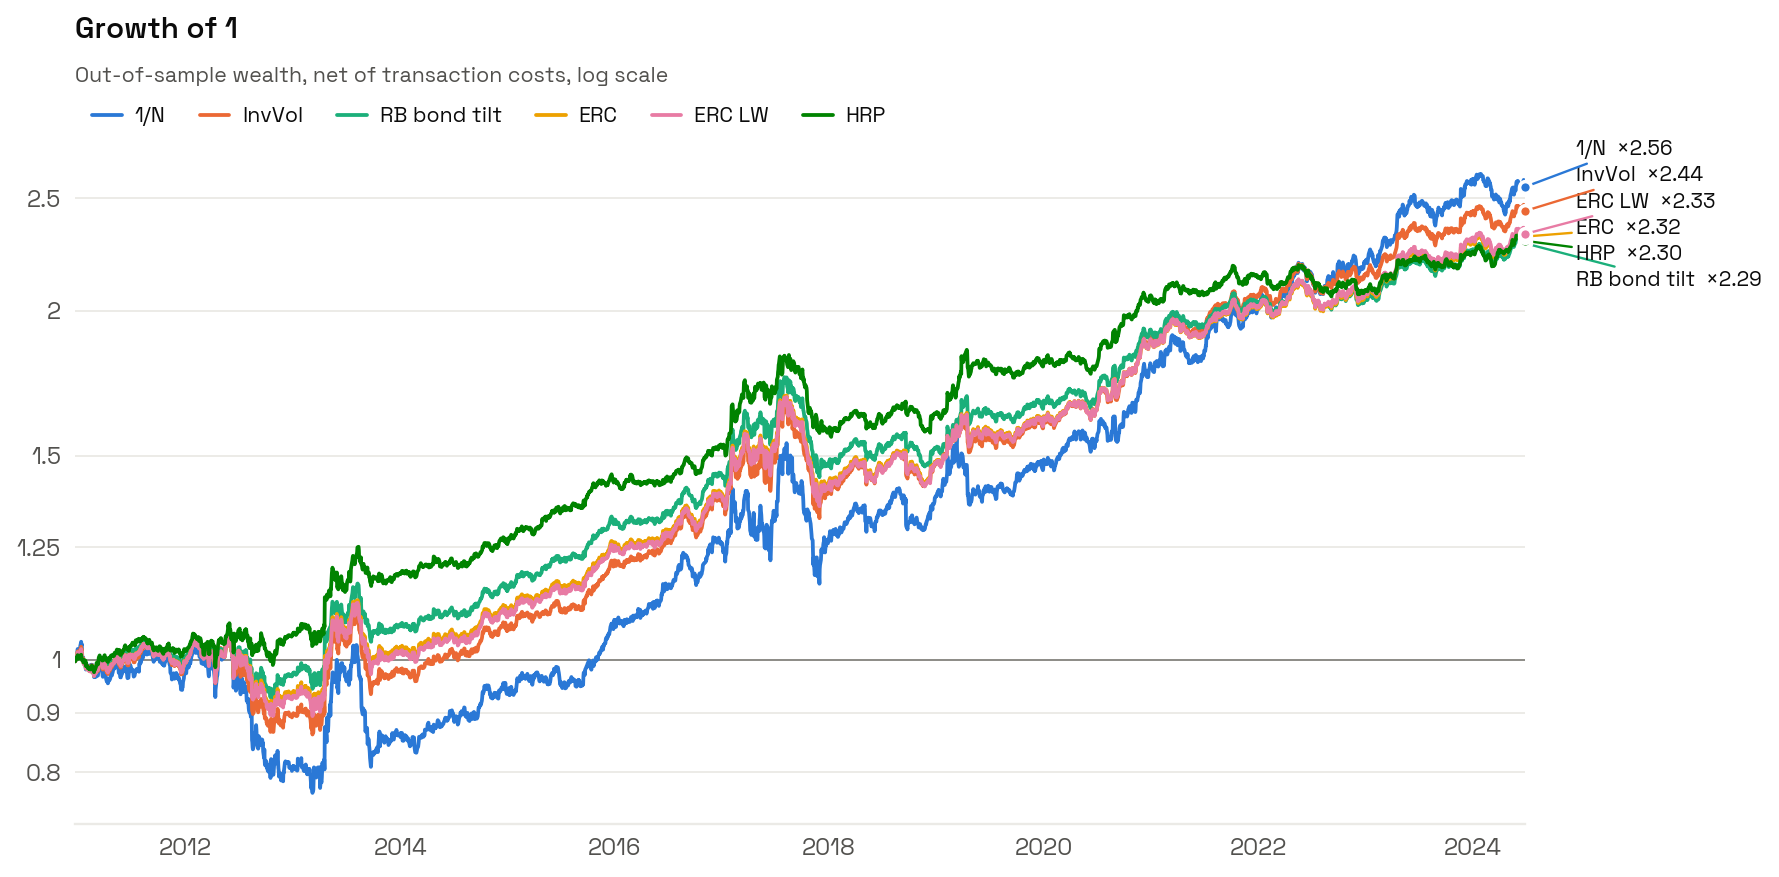
\includegraphics[width=\linewidth]{report_01_wealth.png}

\vspace{1cm}
{\sffamily\small
\begin{tabular}{@{}l@{\hspace{1.2cm}}l@{}}
\color{ink2}Auteur & Jean Philippe N'DRI \\
\color{ink2}Version & Septembre 2026 \\
\color{ink2}Code & \py{portopt/}
\end{tabular}}
\restoregeometry
\end{titlepage}

{\hypersetup{linkcolor=ink}\tableofcontents}
\thispagestyle{fancy}
\newpage

% =============================================================================
\section{Prise en main}\label{sec:start}

\subsection{Ce que fait la librairie}

\py{portopt} répond à une question : \emph{quelle règle d'allocation aurait donné le
meilleur couple rendement/risque, sans utiliser d'information future ?} Elle suit un
flux en quatre étapes, un module par étape.

\begin{center}
\begin{tikzpicture}[
  box/.style={draw=accent,fill=accentsoft,rounded corners=3pt,line width=0.8pt,
    minimum width=2.75cm,minimum height=1.3cm,align=center,font=\sffamily\small},
  lab/.style={font=\scriptsize,text=ink2,align=center},
  arr/.style={-{Stealth[length=6pt]},line width=0.8pt,color=ink2}]
\node[box] (d) {\textbf{data}\\[1pt]{\scriptsize prix $\to$ rendements}};
\node[box,right=1.15cm of d] (e) {\textbf{estimator}\\[1pt]{\scriptsize fenêtre $\to$ poids}};
\node[box,right=1.15cm of e] (b) {\textbf{backtester}\\[1pt]{\scriptsize poids $\to$ rendements}};
\node[box,right=1.15cm of b] (m) {\textbf{metric, plot}\\[1pt]{\scriptsize rendements $\to$ bilan}};
\draw[arr] (d) -- node[above,lab]{$R$} node[below,lab]{$T\times N$} (e);
\draw[arr] (e) -- node[above,lab]{$w$} node[below,lab]{$N$} (b);
\draw[arr] (b) -- node[above,lab]{$R_p$} node[below,lab]{$T-L$} (m);
\end{tikzpicture}
\end{center}

\begin{enumerate}
\item \textbf{data} télécharge des prix, les nettoie et calcule les rendements $R$, un
\py{DataFrame} de $T$ dates par $N$ actifs (section~\ref{sec:data}).
\item \textbf{estimator} transforme une fenêtre de rendements en poids $w$ : c'est la
\emph{règle d'allocation} (sections~\ref{sec:cov} à~\ref{sec:alloc}).
\item \textbf{backtester} applique la règle à chaque date de rebalancement, fait vivre le
portefeuille entre deux dates et renvoie ses rendements hors échantillon $R_p$
(section~\ref{sec:backtest}).
\item \textbf{metric} et \textbf{plot} résument ces rendements en indicateurs et en
graphiques (sections~\ref{sec:perf} à~\ref{sec:stats}).
\end{enumerate}

\subsection{Premier backtest}

\begin{lstlisting}
pip install -e ".[dev]"      # numpy, pandas, scipy, yfinance, matplotlib, pytest
\end{lstlisting}

\begin{lstlisting}
from portopt import load_returns, EqualWeight, ERC, HRP, run_backtests, summary
from portopt import plot

# 1. data : rendements quotidiens, T dates x N actifs
R = load_returns(["SPY", "TLT", "GLD", "DBC", "EFA"], start="2008-01-01")

# 2. estimator : les regles d'allocation a comparer
rules = {"1/N": EqualWeight(), "ERC": ERC(), "HRP": HRP()}

# 3. backtester : fenetre de 252 jours, rebalancement tous les 21 jours
rets, bts = run_backtests(R, rules, in_sample=252, out_of_sample=21,
                          transaction_cost_bps=5)

# 4. metric et plot
print(summary(rets))
plot.save_report(rets, bts, "outputs/charts")
\end{lstlisting}

\py{rets} contient un rendement quotidien hors échantillon par stratégie, et
\py{bts["ERC"].weights_} les poids d'ERC à chaque rebalancement. Sans accès réseau, la
fonction \py{simulate_returns()} du module \py{data} fournit un univers simulé de 10 ETF.

\subsection{Écrire sa propre règle}

Une règle hérite de \py{BaseEstimator} et implémente \py{_compute_weights}. Le
backtester l'accepte telle quelle.

\begin{lstlisting}
import numpy as np
from portopt import BaseEstimator

class InverseVariance(BaseEstimator):
    def _compute_weights(self, returns):
        cov = self._cov(returns)          # applique cov_method
        return 1.0 / np.diag(cov)
\end{lstlisting}

\py{fit} fait le reste : il refuse les fenêtres contenant des valeurs manquantes, met à
zéro les poids négatifs, normalise la somme à 1 et stocke le résultat dans
\py{weights_}, une \py{pd.Series} indexée par actif.

\subsection{Carte de l'API}

\begin{center}\small
\begin{tabularx}{\linewidth}{@{}l>{\raggedright}X>{\raggedright\arraybackslash}p{1.5cm}@{}}
\toprule
Objet & Rôle & Section \\
\midrule
\py{load_returns}, \py{download_prices} & obtenir des prix et des rendements & \ref{sec:data} \\
\py{clean_prices}, \py{compute_returns} & nettoyer, calculer les rendements & \ref{sec:data} \\
\py{simulate_returns} & univers simulé pour travailler hors ligne & \ref{sec:data} \\
\py{estimate_cov}, \py{ledoit_wolf_cov}, \py{ewma_cov} & estimer la covariance & \ref{sec:cov} \\
\py{risk_contributions} & contributions au risque & \ref{sec:rc} \\
\py{EqualWeight}, \py{InverseVolatility} & règles sans optimisation & \ref{sec:ew}, \ref{sec:iv} \\
\py{RiskParity}, \py{ERC} & risk budgeting, contributions égales & \ref{sec:rb}, \ref{sec:erc} \\
\py{HRP} & Hierarchical Risk Parity & \ref{sec:hrp} \\
\py{Backtester}, \py{run_backtests} & backtest walk-forward & \ref{sec:backtest} \\
\py{summary}, module \py{metric} & indicateurs de performance et de risque & \ref{sec:perf}--\ref{sec:stats} \\
\py{plot.save_report} & rapport graphique (PNG) & \ref{sec:example} \\
\bottomrule
\end{tabularx}
\end{center}

\subsection{Notations}

\begin{center}\small
\begin{tabularx}{\linewidth}{@{}>{$}l<{$}X@{}}
\toprule
N,\ T & nombre d'actifs, nombre de dates \\
R_t\in\R^N & rendements simples des actifs, de la clôture $t-1$ à la clôture $t$ \\
\simplex & $\{w\in\R^N : w\ge0,\ \one\T w=1\}$, ensemble des portefeuilles long-only \\
\Sigma,\ \sigma_i,\ \rho_{ij} & covariance, volatilités $\sigma_i=\sqrt{\Sigma_{ii}}$, corrélations \\
P & nombre de périodes par an (252 en quotidien) \\
L,\ H & longueur de la fenêtre d'estimation, période de détention \\
\bar R,\ \hat\sigma & moyenne et écart-type empiriques \\
\Phi,\ \varphi & fonction de répartition et densité de la loi normale centrée réduite \\
\bottomrule
\end{tabularx}
\end{center}

% =============================================================================
\section{Rendements et portefeuille}\label{sec:data}

\begin{definition}[rendements]
Pour un prix $P_t$ ajusté des dividendes et des splits, le rendement simple et le
log-rendement sont
\[
R_t=\frac{P_t}{P_{t-1}}-1,\qquad r_t=\ln\frac{P_t}{P_{t-1}}=\ln(1+R_t).
\]
\end{definition}

\begin{definition}[portefeuille]
Un portefeuille est un vecteur $w\in\simplex$ : $w_i$ est la part de la valeur investie
dans l'actif $i$. On note $R_{p,t}$ son rendement.
\end{definition}

\begin{proposition}\label{prop:simple}
Si $w$ sont les poids en $t-1$, alors $R_{p,t}=w\T R_t$. L'égalité analogue est fausse
pour les log-rendements.
\end{proposition}

\begin{proof}
Soit $n_i$ le nombre de titres $i$ détenus et $V_t=\sum_in_iP_{i,t}$. Alors
$V_t/V_{t-1}=\sum_i\frac{n_iP_{i,t-1}}{V_{t-1}}\cdot\frac{P_{i,t}}{P_{i,t-1}}=\sum_iw_i(1+R_{i,t})$,
d'où $R_{p,t}=w\T R_t$. Pour les log-rendements, $r_{p,t}=\ln\sum_iw_ie^{r_{i,t}}$, qui
est strictement supérieur à $\sum_iw_ir_{i,t}$ dès que les $r_{i,t}$ diffèrent (stricte
concavité du logarithme).
\end{proof}

Toute la librairie travaille donc en \textbf{rendements simples}.

\begin{definition}[volatilité du portefeuille]
Si $\Sigma$ est la covariance des rendements, la variance et la volatilité du
portefeuille $w$ sont $\sigma_p^2(w)=w\T\Sigma w$ et $\sigma_p(w)=\sqrt{w\T\Sigma w}$.
\end{definition}

\begin{definition}[annualisation]
Pour des rendements de fréquence $P$ par an : $\mu_{\mathrm{ann}}=P\,\bar R$ et
$\sigma_{\mathrm{ann}}=\sqrt P\,\hat\sigma$.
\end{definition}

\begin{proposition}\label{prop:annual}
Si les rendements des $P$ périodes d'une année sont indépendants, de moyenne $\mu$ et de
variance $\sigma^2$, et si le rendement annuel est leur somme, alors il a pour moyenne
$P\mu$ et pour écart-type $\sqrt P\,\sigma$.
\end{proposition}

\begin{proof}
L'espérance est linéaire, et par indépendance la variance d'une somme est la somme des
variances : $\Var\bigl(\sum_{k=1}^PX_k\bigr)=P\sigma^2$.
\end{proof}

L'additivité est exacte pour les log-rendements et vraie au premier ordre pour les
rendements simples quotidiens. C'est ce qui justifie les facteurs $P$ et $\sqrt P$.

\begin{code}
\py{load_returns(tickers, start, end, cache_dir="data_cache")} télécharge des prix
ajustés, les nettoie et renvoie des rendements simples. Le nettoyage (\py{clean_prices})
comble les trous d'au plus 5 jours avec la dernière valeur connue, ne comble jamais avec
une valeur future, et conserve les valeurs manquantes d'un actif pas encore coté : le
backtester ne l'investit qu'une fois son historique complet.
\end{code}

% =============================================================================
\section{Estimer la covariance}\label{sec:cov}

Toutes les règles sauf 1/N utilisent une estimation de $\Sigma$ sur la fenêtre.

\begin{definition}[covariance empirique]
Sur une fenêtre de $T$ dates, avec $x_t=R_t-\bar R$ : $S=\frac{1}{T-1}\sum_{t=1}^Tx_tx_t\T$.
\end{definition}

$S$ est sans biais mais bruitée. Elle compte $N(N+1)/2$ paramètres et, si $T\le N$, elle
est de rang au plus $T-1$, donc non inversible.

\begin{theoreme}[Marchenko-Pastur]\label{thm:mp}
Si les $R_t$ sont indépendants de covariance $I_N$ et $N,T\to\infty$ avec $N/T\to q\in(0,1]$,
les valeurs propres de $S$ se répartissent sur $\bigl[(1-\sqrt q)^2,(1+\sqrt q)^2\bigr]$.
\admis{\citealp{marchenko1967}}
\end{theoreme}

Même si toutes les vraies valeurs propres valent 1, celles de $S$ s'étalent de $0.09$ à
$2.91$ pour $q=0.5$. Les petites valeurs propres sont sous-estimées, et ce sont
précisément celles qu'une inversion de $\Sigma$ amplifie.

\begin{definition}[Ledoit-Wolf]
Soit $S_T=\frac1T\sum_tx_tx_t\T$, $\lVert A\rVert^2=\tr(AA\T)/N$ et $\mu=\tr(S_T)/N$. On
pose
\[
d^2=\lVert S_T-\mu I\rVert^2,\quad
\bar b^2=\frac1{T^2}\sum_{t=1}^T\lVert x_tx_t\T-S_T\rVert^2,\quad
\delta^\ast=\frac{\min(\bar b^2,d^2)}{d^2}\in[0,1],\quad
\hat\Sigma=\delta^\ast\mu I+(1-\delta^\ast)S_T .
\]
\end{definition}

$d^2$ mesure l'écart de $S_T$ à la cible $\mu I$, $\bar b^2$ le bruit d'estimation de
$S_T$ ; $\delta^\ast$ est la part de l'écart attribuée au bruit. Ce choix minimise
asymptotiquement l'erreur quadratique parmi les combinaisons de $S_T$ et $\mu I$
\admis{\citealp{ledoitwolf2004}}.

\begin{proposition}\label{prop:lw}
Soit $\lambda_1\ge\dots\ge\lambda_N$ les valeurs propres de $S_T$ et $\delta^\ast>0$.
\begin{enumerate}[label=(\roman*)]
\item $\hat\Sigma$ a les mêmes vecteurs propres que $S_T$, pour valeurs propres
$\delta^\ast\mu+(1-\delta^\ast)\lambda_j$, et elle est définie positive.
\item Son conditionnement $\lambda_{\max}/\lambda_{\min}$ est inférieur à celui de $S_T$.
\end{enumerate}
\end{proposition}

\begin{proof}
(i) Si $S_Tv=\lambda v$, alors $\hat\Sigma v=(\delta^\ast\mu+(1-\delta^\ast)\lambda)v$, et
ces valeurs sont au moins $\delta^\ast\mu>0$.
(ii) Avec $a=\delta^\ast\mu>0$ et $c=1-\delta^\ast$, l'inégalité
$\frac{a+c\lambda_1}{a+c\lambda_N}\le\frac{\lambda_1}{\lambda_N}$ équivaut à
$a\lambda_N\le a\lambda_1$, qui est vraie.
\end{proof}

\begin{lemme}[calcul de $\bar b^2$ sans former les $x_tx_t\T$]
$\sum_t\lVert x_tx_t\T-S_T\rVert_F^2=\sum_t(x_t\T x_t)^2-T\lVert S_T\rVert_F^2$.
\end{lemme}

\begin{proof}
$\lVert x_tx_t\T-S_T\rVert_F^2=(x_t\T x_t)^2-2x_t\T S_Tx_t+\lVert S_T\rVert_F^2$, et
$\sum_tx_t\T S_Tx_t=\tr\bigl(S_T\sum_tx_tx_t\T\bigr)=T\lVert S_T\rVert_F^2$.
\end{proof}

\fig[0.92\linewidth]{lw_spectrum.png}{Valeurs propres de la vraie covariance, de la
covariance empirique et de Ledoit-Wolf (50 actifs, 75 dates). Le shrinkage remonte les
petites valeurs propres et divise le conditionnement par 5.}

\begin{definition}[EWMA]
Pour une demi-vie $h$, on pose $\lambda=2^{-1/h}$ et $\omega_s=\lambda^s/\sum_u\lambda^u$,
$s=0$ désignant la date la plus récente. Alors
$\hat\Sigma=\sum_s\omega_s(R_{t-s}-\bar R_\omega)(R_{t-s}-\bar R_\omega)\T$, avec
$\bar R_\omega=\sum_s\omega_sR_{t-s}$.
\end{definition}

\begin{proposition}
Sur un historique infini, le nombre effectif d'observations
$(\sum_s\omega_s)^2/\sum_s\omega_s^2$ vaut $(1+\lambda)/(1-\lambda)$, soit environ 182
pour $h=63$.
\end{proposition}

\begin{proof}
$\sum_s\lambda^s=\frac1{1-\lambda}$ et $\sum_s\lambda^{2s}=\frac1{1-\lambda^2}$, donc le
rapport vaut $\frac{1-\lambda^2}{(1-\lambda)^2}=\frac{1+\lambda}{1-\lambda}$.
\end{proof}

\begin{code}
Toute règle accepte \py{cov_method="sample" | "ledoit_wolf" | "ewma"} ou une fonction
\py{returns -> ndarray}. Directement : \py{estimate_cov(R, "ledoit_wolf")},
\py{ledoit_wolf_cov(R)} qui renvoie \py{(Sigma, delta)}, \py{ewma_cov(R, halflife=63)}.
\end{code}

\begin{pratique}
Aucune règle de la librairie n'utilise les rendements espérés. L'erreur standard d'une
moyenne annualisée vaut $\sigma/\sqrt Y$ sur $Y$ années, quelle que soit la fréquence
($\pm5\pct$ pour $\sigma=16\pct$ et 10 ans), alors que l'erreur sur une variance diminue
avec le nombre d'observations : la covariance s'estime bien mieux que la moyenne.
\end{pratique}

% =============================================================================
\section{Contributions au risque}\label{sec:rc}

\begin{proposition}[décomposition d'Euler]\label{prop:euler}
Pour tout $w$ tel que $\sigma_p(w)>0$ :
$\dfrac{\partial\sigma_p}{\partial w}=\dfrac{\Sigma w}{\sigma_p}$ et
$\sigma_p(w)=\sum_{i=1}^Nw_i\,\dfrac{\partial\sigma_p}{\partial w_i}(w)$.
\end{proposition}

\begin{proof}
Le gradient s'obtient en dérivant $\sqrt{w\T\Sigma w}$. Puis
$\sum_iw_i(\Sigma w)_i/\sigma_p=w\T\Sigma w/\sigma_p=\sigma_p$.
\end{proof}

\begin{definition}[contributions au risque]
Contribution marginale, contribution et contribution relative de l'actif $i$ :
\[
\MRC_i=\frac{(\Sigma w)_i}{\sigma_p},\qquad\RC_i=w_i\MRC_i,\qquad
\frac{\RC_i}{\sigma_p}=\frac{w_i(\Sigma w)_i}{w\T\Sigma w}.
\]
Par la proposition~\ref{prop:euler}, les $\RC_i$ somment à $\sigma_p$ et les
contributions relatives à 1.
\end{definition}

\begin{proposition}\label{prop:beta}
$\MRC_i=\beta_{i,p}\,\sigma_p=\rho_{i,p}\,\sigma_i$, où $\beta_{i,p}$ et $\rho_{i,p}$ sont
le bêta et la corrélation de l'actif $i$ avec le portefeuille.
\end{proposition}

\begin{proof}
$(\Sigma w)_i=\Cov(R_i,w\T R)=\Cov(R_i,R_p)$. Avec
$\beta_{i,p}=\Cov(R_i,R_p)/\sigma_p^2$ et $\rho_{i,p}=\Cov(R_i,R_p)/(\sigma_i\sigma_p)$, on
obtient les deux égalités.
\end{proof}

Un actif pèse dans le risque par son bêta au portefeuille, pas par sa volatilité propre.
S'il est négativement corrélé au portefeuille, sa contribution est négative.

\begin{exemple}
60/40 actions/obligations, $\sigma_A=16\pct$, $\sigma_O=6\pct$, $\rho=-0.2$ :
$\sigma_p^2=0.36\cdot0.0256+0.16\cdot0.0036-0.48\cdot0.2\cdot0.0096=0.00887$, soit
$\sigma_p=9.4\pct$. Puis $(\Sigma w)_A=0.6\cdot0.0256-0.4\cdot0.00192=0.01459$ et
$\RC_A/\sigma_p=0.6\cdot0.01459/0.00887=98.7\pct$ : un 60/40 en capital est un 99/1 en
risque.
\end{exemple}

\begin{code}
\py{risk_contributions(w, cov)} renvoie les contributions relatives ;
\py{Backtester.risk_contributions()} les donne à chaque rebalancement.
\end{code}

% =============================================================================
\section{Règles d'allocation}\label{sec:alloc}

\begin{definition}[règle d'allocation]
Une règle d'allocation est une fonction $\mathcal A$ qui associe à une fenêtre de
rendements $(R_{t-L},\dots,R_{t-1})$ un portefeuille $w\in\simplex$. Dans la librairie,
c'est un \py{BaseEstimator} : \py{est.fit(fenetre).weights_}.
\end{definition}

% -----------------------------------------------------------------------------
\subsection{Equal Weight (1/N)}\label{sec:ew}

\begin{definition}
$w_i=1/N$ pour tout $i$.
\end{definition}

\begin{proposition}\label{prop:ew}
Si tous les actifs ont la volatilité $\sigma$ et des corrélations deux à deux égales à
$\rho$, alors
$\sigma_{1/N}^2=\frac{\sigma^2}{N}\bigl(1+(N-1)\rho\bigr)\to\rho\sigma^2$ quand $N\to\infty$.
\end{proposition}

\begin{proof}
$w\T\Sigma w=\frac1{N^2}\bigl(N\sigma^2+N(N-1)\rho\sigma^2\bigr)$.
\end{proof}

La diversification supprime le risque propre à chaque actif mais pas le risque commun
$\rho\sigma^2$. 1/N n'estime rien et ne commet donc aucune erreur d'estimation : c'est
le benchmark de référence, qu'aucun des 14 modèles d'optimisation testés par
\citet{demiguel2009} ne bat significativement hors échantillon.

\begin{code}
\py{EqualWeight()}
\end{code}

% -----------------------------------------------------------------------------
\subsection{Inverse volatilité}\label{sec:iv}

\begin{definition}
$w_i=\sigma_i^{-k}/\sum_j\sigma_j^{-k}$, avec $k=1$ (inverse volatilité) ou $k=2$
(inverse variance).
\end{definition}

\begin{proposition}\label{prop:invvol}
\begin{enumerate}[label=(\roman*)]
\item Si toutes les corrélations sont égales, l'inverse volatilité égalise les
contributions au risque : c'est l'ERC (section~\ref{sec:erc}).
\item Si $\Sigma$ est diagonale, l'inverse variance est le portefeuille de variance
minimale.
\end{enumerate}
\end{proposition}

\begin{proof}
(i) Avec $w_i=c/\sigma_i$ et $\rho_{ij}=\rho$ pour $i\ne j$ :
$(\Sigma w)_i=\sum_j\rho_{ij}\sigma_i\sigma_j\,c/\sigma_j=c\,\sigma_i\bigl(1+(N-1)\rho\bigr)$,
donc $w_i(\Sigma w)_i=c^2\bigl(1+(N-1)\rho\bigr)$ ne dépend pas de $i$.
(ii) Le portefeuille de variance minimale est $w\propto\Sigma^{-1}\one$ et, pour $\Sigma$
diagonale, $\Sigma^{-1}\one=(\sigma_i^{-2})_i$.
\end{proof}

\begin{code}
\py{InverseVolatility(exponent=1)} ; \py{exponent=2} pour l'inverse variance.
\end{code}

% -----------------------------------------------------------------------------
\subsection{Risk budgeting}\label{sec:rb}

\begin{definition}
Soit des budgets $b_i>0$ de somme 1. Un portefeuille de risk budgeting est un
$w\in\simplex$ tel que $w_i(\Sigma w)_i/(w\T\Sigma w)=b_i$ pour tout $i$ : l'actif $i$
porte la part $b_i$ du risque.
\end{definition}

\begin{theoreme}[\citealp{spinu2013}]\label{thm:spinu}
Soit $\Sigma\succ0$ et $f(y)=\frac12y\T\Sigma y-\sum_ib_i\ln y_i$ sur $\R^N_{++}$. Alors $f$
a un unique minimiseur $y^\ast$, et $w^\ast=y^\ast/\one\T y^\ast$ est l'unique
portefeuille de risk budgeting.
\end{theoreme}

\begin{proof}
\emph{Existence.} $f\to+\infty$ quand un $y_i\to0^+$ (terme logarithmique) et quand
$\lVert y\rVert\to\infty$ (le terme quadratique, minoré par
$\frac12\lambda_{\min}(\Sigma)\lVert y\rVert^2$, domine). Le minimum est donc atteint à
l'intérieur de $\R^N_{++}$.
\emph{Unicité.} $\nabla^2f=\Sigma+\diag(b_i/y_i^2)\succ0$ : $f$ est strictement convexe.
\emph{Budgets.} $\partial_if=(\Sigma y)_i-b_i/y_i=0$ donne $y^\ast_i(\Sigma y^\ast)_i=b_i$.
Comme $w_i(\Sigma w)_i$ est homogène de degré 2, les contributions relatives de $w^\ast$
valent $b_i/\sum_jb_j=b_i$.
\emph{Unicité du portefeuille.} Si $w$ convient, $y=w/\sqrt{w\T\Sigma w}$ vérifie
$y_i(\Sigma y)_i=b_i$, donc $\nabla f(y)=0$, donc $y=y^\ast$.
\end{proof}

\begin{proposition}[mise à jour par coordonnée]\label{prop:ccd}
À $(y_j)_{j\ne i}$ fixés, le minimiseur de $f$ en $y_i>0$ est
\[
y_i=\frac{-c_i+\sqrt{c_i^2+4\Sigma_{ii}b_i}}{2\Sigma_{ii}},\qquad c_i=\sum_{j\ne i}\Sigma_{ij}y_j .
\]
\end{proposition}

\begin{proof}
$\partial_if=0$ s'écrit $\Sigma_{ii}y_i^2+c_iy_i-b_i=0$. Le produit des racines,
$-b_i/\Sigma_{ii}$, est négatif : une seule racine est positive, et c'est celle-ci.
\end{proof}

En répétant cette mise à jour sur $i=1,\dots,N$ jusqu'à stabilisation (descente par
coordonnées cyclique), on converge vers $y^\ast$ \admis{\citealp{tseng2001}}.

\begin{algorithm}[H]
\caption{Risk budgeting par descente par coordonnées (\py{RiskParity})}\label{alg:ccd}
\KwIn{$\Sigma\succ0$, budgets $b$, tolérance $\varepsilon=10^{-10}$}
\KwOut{poids $w$}
$y_i\gets b_i/\sigma_i$ ; \quad $y\gets y/\sqrt{y\T\Sigma y}$ ; \quad $s\gets\Sigma y$\;
\Repeat{$\lVert y-y^{\mathrm{old}}\rVert\le\varepsilon\lVert y\rVert$}{
  $y^{\mathrm{old}}\gets y$\;
  \For{$i\gets1$ \KwTo $N$}{
    $c\gets s_i-\Sigma_{ii}y_i$ ; \quad $y_i'\gets\bigl(-c+\sqrt{c^2+4\Sigma_{ii}b_i}\bigr)/(2\Sigma_{ii})$\;
    $s\gets s+\Sigma_{:,i}(y_i'-y_i)$ ; \quad $y_i\gets y_i'$ \Com*[r]{coût $O(N)$, sans inversion}
  }
}
\KwRet{$w=y/\one\T y$}
\end{algorithm}

\begin{code}
\py{RiskParity(budgets={"SPY": 1, "TLT": 2, ...})}, un budget strictement positif par
actif (normalisés automatiquement) ; \py{n_iter_} donne le nombre de cycles.
\end{code}

% -----------------------------------------------------------------------------
\subsection{Equal Risk Contribution (ERC)}\label{sec:erc}

\begin{definition}
L'ERC est le risk budgeting avec $b_i=1/N$ : chaque actif porte la même part du risque.
\end{definition}

\begin{theoreme}[\citealp{maillard2010}]\label{thm:erc}
Si $\sMV$ est la volatilité du portefeuille long-only de variance minimale, alors
$\sMV\le\sERC\le\sEW$.
\end{theoreme}

\begin{proof}
La première inégalité vient de ce que le min-variance minimise $\sigma_p$ sur tout
$\simplex$. Pour la seconde, $\sigma_p$ est convexe (norme de $\Sigma^{1/2}w$), donc
au-dessus de sa tangente en $w=w_{\mathrm{ERC}}$. Avec $\nabla\sigma_p(w)\T w=\sigma_p(w)$
(proposition~\ref{prop:euler}) :
\[
\sEW\ \ge\ \sERC+\nabla\sigma_p(w)\T\bigl(\tfrac{\one}{N}-w\bigr)=\frac1N\sum_i\partial_i\sigma_p(w).
\]
En ERC, $w_i\,\partial_i\sigma_p=\sERC/N$, d'où
$\sEW\ge\frac{\sERC}{N^2}\sum_i\frac1{w_i}\ge\sERC$, car $\sum_i1/w_i\ge N^2$ sur
$\simplex$ (inégalité arithmético-harmonique).
\end{proof}

\begin{proposition}\label{prop:tangent}
Si tous les actifs ont le même ratio de Sharpe et des corrélations égales, l'ERC est le
portefeuille de Sharpe maximal.
\end{proposition}

\begin{proof}
Le portefeuille de Sharpe maximal est $w\propto\Sigma^{-1}\mu$. Avec $\mu_i=s\sigma_i$,
$\Sigma=DCD$, $D=\diag(\sigma_i)$ et $C=(1-\rho)I+\rho\one\one\T$ : comme
$C\one=(1+(N-1)\rho)\one$, on a $\Sigma^{-1}\mu=sD^{-1}C^{-1}\one\propto D^{-1}\one$. C'est
l'inverse volatilité, égale à l'ERC par la proposition~\ref{prop:invvol}.
\end{proof}

\fig[0.95\linewidth]{erc_two_assets.png}{Deux actifs ($\sigma_1=18\pct$, $\sigma_2=6\pct$,
$\rho=-0.2$). L'ERC a une volatilité proche du minimum (5.7\pct{} contre 5.3\pct) mais
répartit le risque à parts égales, alors que 1/N en met 95\pct{} sur l'actif risqué.}

\begin{code}
\py{ERC(cov_method="ledoit_wolf")}
\end{code}

% -----------------------------------------------------------------------------
\subsection{Hierarchical Risk Parity (HRP)}\label{sec:hrp}

HRP \citep{lopezdeprado2016} regroupe les actifs qui se ressemblent, puis répartit le
capital entre groupes avant de le répartir dans chaque groupe. Il n'inverse jamais
$\Sigma$.

\begin{definition}[distance de corrélation]
$d_{ij}=\sqrt{\tfrac12(1-\rho_{ij})}\in[0,1]$.
\end{definition}

\begin{proposition}
$d$ est une distance, nulle si et seulement si $\rho_{ij}=1$.
\end{proposition}

\begin{proof}
Soit $z_i$ la série de l'actif $i$ centrée et de norme 1. Alors $\rho_{ij}=z_i\T z_j$ et
$\lVert z_i-z_j\rVert^2=2-2\rho_{ij}$, donc $d_{ij}=\frac12\lVert z_i-z_j\rVert$ hérite
des propriétés de la norme euclidienne.
\end{proof}

\begin{definition}[HRP]
\begin{enumerate}
\item \emph{Clustering} : classification hiérarchique des actifs selon $d$ (méthode
\py{linkage}), qui produit un arbre binaire.
\item \emph{Quasi-diagonalisation} : on ordonne les actifs selon les feuilles de l'arbre,
ce qui place côte à côte les actifs corrélés.
\item \emph{Bissection} : on part de $w=\one$ et on découpe récursivement chaque groupe
en deux sous-groupes $L$ et $R$ (deux moitiés de la liste ordonnée, ou les deux branches
de l'arbre). À chaque découpe,
\[
\alpha=\frac{V_R}{V_L+V_R},\qquad w_L\leftarrow\alpha\,w_L,\qquad w_R\leftarrow(1-\alpha)\,w_R,
\]
où $V_c=\tilde w_c\T\Sigma_c\tilde w_c$ est la variance du portefeuille inverse variance
du groupe $c$, avec $\tilde w_c\propto\diag(\Sigma_c)^{-1}$.
\end{enumerate}
\end{definition}

Chaque sous-groupe reçoit une part inversement proportionnelle à sa variance. Les
$\tilde w_c$ servent uniquement à calculer $V_c$ : les poids finaux résultent des
découpes successives, jusqu'aux actifs individuels.

\fig{hrp_steps.png}{Étapes de HRP sur l'univers simulé : corrélations dans un ordre
arbitraire, arbre, corrélations réordonnées. Deux blocs apparaissent : taux et crédit en
haut, actifs risqués en bas.}

\begin{proposition}\label{prop:hrp}
\begin{enumerate}[label=(\roman*)]
\item HRP renvoie un portefeuille de $\simplex$ et n'inverse que des diagonales : il
fonctionne même si $\Sigma$ est singulière.
\item Si $\Sigma$ est diagonale, HRP est le portefeuille inverse variance.
\end{enumerate}
\end{proposition}

\begin{proof}
(i) Avant qu'un groupe $c$ soit découpé, tous ses actifs portent le même poids $m_c$
(ils ont subi les mêmes multiplications), avec $m=1$ pour l'univers entier. Une découpe
donne $m_L=\alpha m_c$ et $m_R=(1-\alpha)m_c$ avec $\alpha\in(0,1)$ puisque $V_L,V_R>0$.
Par récurrence sur l'arbre, la somme des poids finaux des actifs de $c$ vaut $m_c$ : pour
un actif seul c'est immédiat, et sinon elle vaut $m_L+m_R=m_c$. Pour l'univers, la somme
vaut 1 et tous les poids sont positifs.
(ii) Pour $\Sigma$ diagonale, $V_c=1/S_c$ avec $S_c=\sum_{i\in c}\sigma_i^{-2}$, donc
$\alpha=S_L/(S_L+S_R)$ : chaque groupe reçoit la part d'inverse variance de ses actifs, et
par récurrence l'actif $i$ reçoit $\sigma_i^{-2}/\sum_j\sigma_j^{-2}$.
\end{proof}

\begin{code}
\py{HRP(linkage="single", split="bisection")} reproduit l'article original ;
\py{split="dendrogram"} suit les branches de l'arbre au lieu de couper la liste en deux
moitiés. Attributs : \py{order_} (ordre des feuilles), \py{linkage_matrix_} (arbre).
\end{code}

\begin{pratique}
L'arbre peut changer d'un rebalancement à l'autre : HRP est plus instable qu'ERC (turnover
2.5 fois plus élevé dans l'exemple). Les méthodes \py{"average"} ou \py{"ward"} donnent des
arbres plus stables que \py{"single"}.
\end{pratique}

% -----------------------------------------------------------------------------
\subsection{Synthèse}

\begin{center}\small
\begin{tabularx}{\linewidth}{@{}l>{\raggedright}X>{\raggedright}X>{\raggedright}X>{\raggedright\arraybackslash}X@{}}
\toprule
& 1/N & InvVol & Risk budgeting, ERC & HRP \\
\midrule
Utilise $\sigma_i$ & non & oui & oui & oui \\
Utilise $\rho_{ij}$ & non & non & oui & oui, via l'arbre \\
Inverse $\Sigma$ & non & non & non & non \\
Calcul & direct & direct & itératif, solution unique & direct \\
Ce qui est égalisé & le capital & $w_i\sigma_i$ & $w_i(\Sigma w)_i$ & la variance entre groupes \\
Résultats & prop.~\ref{prop:ew} & prop.~\ref{prop:invvol} & th.~\ref{thm:spinu}, \ref{thm:erc} & prop.~\ref{prop:hrp} \\
\bottomrule
\end{tabularx}
\end{center}

% =============================================================================
\section{Backtest walk-forward}\label{sec:backtest}

\begin{definition}[backtest walk-forward]
Soit une règle $\mathcal A$, une fenêtre $L$ et une période de détention $H$. Les dates
de rebalancement sont $t_k=L+kH$. À chaque $t_k$, on calcule
$w^{(k)}=\mathcal A(R_{t_k-L},\dots,R_{t_k-1})$ (fenêtre glissante) ou
$\mathcal A(R_0,\dots,R_{t_k-1})$ (fenêtre croissante), puis on détient ce portefeuille
jusqu'à $t_{k+1}-1$.
\end{definition}

\fig[0.95\linewidth]{walk_forward.png}{Estimation sur $[t-L,t)$, détention sur $[t,t+H)$,
puis décalage de $H$.}

\begin{proposition}[absence d'anticipation]
Le portefeuille qui gagne le rendement $R_t$ ne dépend que de $R_0,\dots,R_{t-1}$.
\end{proposition}

\begin{proof}
Si $t_k\le t<t_{k+1}$, $R_t$ est gagné avec $w^{(k)}$ dérivé jusqu'en $t-1$ (définition
ci-dessous). $w^{(k)}$ ne dépend que de rendements antérieurs à $t_k\le t$, et la dérive
que de $R_{t_k},\dots,R_{t-1}$.
\end{proof}

\begin{definition}[dérive des poids]
Entre deux rebalancements, les quantités détenues ne changent pas. $k$ jours après le
rebalancement ($V_0=1$) :
\[
V_k=\sum_iw_i\prod_{s=1}^k(1+R_{i,s}),\qquad R_{p,k}=\frac{V_k}{V_{k-1}}-1 .
\]
\end{definition}

\begin{proposition}\label{prop:drift}
Le poids de l'actif $i$ après $k$ jours est $w_i^{(k)}=w_i\prod_{s\le k}(1+R_{i,s})/V_k$,
et $R_{p,k}=\sum_iw_i^{(k-1)}R_{i,k}$.
\end{proposition}

\begin{proof}
La ligne $i$ vaut $w_i\prod_{s\le k}(1+R_{i,s})$ et son poids est cette valeur divisée par
$V_k$. Ensuite
$\frac{V_k}{V_{k-1}}=\sum_i\frac{w_i\prod_{s<k}(1+R_{i,s})}{V_{k-1}}(1+R_{i,k})=\sum_iw_i^{(k-1)}(1+R_{i,k})$ :
c'est la proposition~\ref{prop:simple} avec les poids dérivés.
\end{proof}

\begin{definition}[turnover et coûts]
Au rebalancement, le turnover est $\tau=\sum_i|w_i^{\mathrm{cible}}-w_i^{\mathrm{dérivé}}|$,
mesuré par rapport aux poids \emph{dérivés} et non à la cible précédente. Avec un coût
proportionnel $c$, la richesse est multipliée par $1-c\,\tau$. Le turnover annualisé est
la somme des $\tau$, hors construction initiale, divisée par le nombre d'années.
\end{definition}

Le coût annuel vaut donc environ $c$ fois le turnover annualisé : 120\pct{} de turnover à
10~bps coûtent 12~bps par an.

\begin{algorithm}[H]
\caption{Backtest walk-forward (\py{Backtester.run})}\label{alg:bt}
\KwIn{rendements $R$, règle $\mathcal A$, $L$, $H$, coût $c$}
\KwOut{rendements hors échantillon nets de coûts}
$w^{\mathrm{dérivé}}\gets0$ ; \quad $t\gets L$ \Com*[r]{départ en cash}
\While{$t<T$}{
  actifs éligibles $\gets$ actifs sans valeur manquante sur la fenêtre\;
  $w\gets\mathcal A(\text{fenêtre})$ ; \quad $\tau\gets\sum_i|w_i-w_i^{\mathrm{dérivé}}|$\;
  détenir $w$ sur $[t,t+H)$ avec dérive ; richesse $\times(1-c\tau)$ en $t$\;
  $w^{\mathrm{dérivé}}\gets$ poids en fin de période ; \quad $t\gets t+H$\;
}
\end{algorithm}

\begin{code}
\py{bt = Backtester(R, ERC(), in_sample=252, out_of_sample=21, transaction_cost_bps=5)} ;
\py{bt.run()} renvoie les rendements nets. Attributs \py{weights_}, \py{turnover_},
\py{gross_returns_} ; méthodes \py{annualized_turnover()} et \py{risk_contributions()}.
Options : \py{window="expanding"}, \py{drift=False} (rebalancement quotidien gratuit vers
la cible). \py{run_backtests} compare plusieurs règles sur la même grille.
\end{code}

% =============================================================================
\section{Indicateurs de performance}\label{sec:perf}

Les fonctions de \py{portopt.metric} prennent une série de rendements simples
(\py{pd.Series}) ou un tableau avec une colonne par stratégie (\py{pd.DataFrame}).

\begin{definition}[rendement total, CAGR]
$\mathrm{TR}=\prod_{t=1}^T(1+R_t)-1$ et $\CAGR=(1+\mathrm{TR})^{P/T}-1$ : le taux annuel
constant qui mène à la même richesse finale.
\end{definition}

\begin{proposition}[volatility drag]\label{prop:drag}
Le taux de croissance $g=\ln(1+\CAGR)$ vérifie, au second ordre,
$g\approx\mu_{\mathrm{ann}}-\frac12\sigma_{\mathrm{ann}}^2$.
\end{proposition}

\begin{proof}
$g=\frac PT\sum_t\ln(1+R_t)$ et $\ln(1+R)=R-\frac{R^2}2+O(R^3)$. Comme
$\frac1T\sum_tR_t^2=\hat\sigma^2+\bar R^2\approx\hat\sigma^2$ en quotidien,
$g\approx P\bar R-\frac P2\hat\sigma^2=\mu_{\mathrm{ann}}-\frac12\sigma_{\mathrm{ann}}^2$.
\end{proof}

À moyenne égale, la stratégie la moins volatile finit plus riche. Dans l'exemple, 1/N a
$\mu_{\mathrm{ann}}=7.36\pct$ et $\sigma_{\mathrm{ann}}=11.42\pct$ : la formule donne
$g=6.71\pct$, pour $6.70\pct$ observé.

\begin{definition}[ratio de Sharpe]
Avec un taux sans risque annuel $r_f$ converti par période,
$\SR=\sqrt P\;\overline{(R-r_f)}\,/\,\hat\sigma$.
\end{definition}

\begin{proposition}\label{prop:srlev}
Le Sharpe est invariant au levier : multiplier les rendements excédentaires par $k>0$ ne
le change pas. Sous les hypothèses de la proposition~\ref{prop:annual}, le Sharpe annuel
vaut $\sqrt P$ fois le Sharpe par période.
\end{proposition}

\begin{proof}
La moyenne et l'écart-type de $kX$ valent $k$ fois ceux de $X$. En annuel, le ratio
devient $P\mu/(\sqrt P\sigma)=\sqrt P\,\mu/\sigma$.
\end{proof}

\begin{definition}[ratio de Sortino]
Pour un seuil $\tau$ par période,
\[
\mathrm{Sortino}=\sqrt P\,\frac{\overline{R-\tau}}{DD_\tau},\qquad
DD_\tau=\sqrt{\frac1T\sum_{t=1}^T\min(R_t-\tau,0)^2}.
\]
La moyenne des carrés porte sur \emph{toutes} les dates, les gains comptant pour zéro.
Le Sortino est le rendement moyen par unité de risque de baisse.
\end{definition}

\begin{proposition}\label{prop:sortino}
\begin{enumerate}[label=(\roman*)]
\item Pour $\tau=0$, le Sortino est invariant au levier.
\item Si $R\sim\mathcal N(\mu,\sigma^2)$, $\tau=0$ et $m=\mu/\sigma$ :
\[
\frac{\mathrm{Sortino}}{\SR}=\frac{1}{\sqrt{(1+m^2)\,\Phi(-m)-m\,\varphi(m)}}
=\sqrt2\,\Bigl(1+\sqrt{2/\pi}\;m\Bigr)+O(m^2).
\]
\end{enumerate}
\end{proposition}

\begin{proof}
(i) Pour $k>0$, $\min(kR,0)=k\min(R,0)$ : numérateur et dénominateur sont multipliés par
$k$.
(ii) Le rapport vaut $\sigma/DD_0$. Avec $R=\sigma(m+Z)$ et $Z\sim\mathcal N(0,1)$,
$DD_0^2=\sigma^2\E\bigl[(m+Z)^2\one_{Z<-m}\bigr]$. Les identités
$\E[Z\one_{Z<a}]=-\varphi(a)$ et $\E[Z^2\one_{Z<a}]=\Phi(a)-a\varphi(a)$, prises en $a=-m$,
donnent $m^2\Phi(-m)-2m\varphi(m)+\Phi(-m)+m\varphi(m)$, d'où la formule. Pour le
développement, $\Phi(-m)=\frac12-\varphi(0)m+O(m^2)$ et $\varphi(m)=\varphi(0)+O(m^2)$ avec
$\varphi(0)=1/\sqrt{2\pi}$, donc le radicande vaut $\frac12-2\varphi(0)m+O(m^2)$.
\end{proof}

Pour une loi symétrique, le Sortino vaut donc environ $\sqrt2\approx1.41$ fois le Sharpe
si la moyenne est nulle, un peu plus si elle est positive. Dans l'exemple (Sharpe
quotidien de 0.04 à 0.055), une gaussienne donnerait 1.46 à 1.48 ; on observe 1.44 à 1.51.
Le Sortino n'apporte alors presque rien de plus que le Sharpe. Il devient informatif
pour des stratégies nettement asymétriques.

\begin{definition}[Calmar, hit ratio]
$\mathrm{Calmar}=\CAGR/|\MaxDD|$ (MaxDD défini en section~\ref{sec:risk}) et
$\mathrm{Hit}=\frac1T\sum_t\one_{R_t>0}$.
\end{definition}

\begin{code}
\py{cagr}, \py{annualized_mean}, \py{annualized_volatility},
\py{sharpe_ratio(r, rf=0.0)} ($r_f$ annuel), \py{sortino_ratio(r, target=0.0)} (seuil
\emph{par période}), \py{calmar_ratio}, \py{hit_ratio}. \py{summary(rets)} les réunit
dans un tableau.
\end{code}

% =============================================================================
\section{Indicateurs de risque}\label{sec:risk}

\begin{definition}[drawdown]
Avec la richesse $W_t=\prod_{s\le t}(1+R_s)$ et $W_0=1$ :
\[
DD_t=\frac{W_t}{\max\bigl(1,\max_{s\le t}W_s\bigr)}-1,\qquad\MaxDD=\min_tDD_t .
\]
La durée maximale sous l'eau est la plus longue suite de dates consécutives où $DD_t<0$.
\end{definition}

Le capital initial compte comme un sommet : perdre 10\pct{} le premier jour donne un
drawdown de $-10\pct$.

\begin{proposition}
Après une perte $\ell\in(0,1)$, il faut un gain $\ell/(1-\ell)$ pour revenir au niveau
initial.
\end{proposition}

\begin{proof}
$(1-\ell)(1+g)=1\iff g=\ell/(1-\ell)$. Ainsi $-20\pct$ demande $+25\pct$, et $-50\pct$
demande $+100\pct$.
\end{proof}

\fig[0.95\linewidth]{drawdown_anatomy.png}{Sommet, creux, récupération et durée sous l'eau
du plus grand drawdown du portefeuille 1/N.}

Le MaxDD s'aggrave mécaniquement avec la durée observée : pour un mouvement brownien sans
dérive, son espérance croît comme $\sigma\sqrt T$ \admis{\citealp{magdonismail2004}}. On
ne compare donc des MaxDD que sur une même période.

\begin{definition}[VaR et CVaR historiques]
Avec $q_\alpha$ le quantile empirique d'ordre $\alpha$ des rendements :
$\VaR_\alpha=-q_\alpha$ et $\CVaR_\alpha=-\E[R\mid R\le q_\alpha]$, exprimées en pertes
positives. La CVaR est la perte moyenne sur la fraction $\alpha$ des pires dates.
\end{definition}

\begin{proposition}\label{prop:var}
\begin{enumerate}[label=(\roman*)]
\item $\CVaR_\alpha\ge\VaR_\alpha$.
\item La VaR n'est pas sous-additive : on peut avoir $\VaR(A+B)>\VaR(A)+\VaR(B)$.
\item La CVaR est sous-additive ; c'est une mesure de risque cohérente
\admis{\citealp{artzner1999}}.
\end{enumerate}
\end{proposition}

\begin{proof}
(i) Sur l'événement $\{R\le q_\alpha\}$, $-R\ge-q_\alpha$ ; on prend l'espérance
conditionnelle.
(ii) Deux obligations indépendantes perdent chacune 100 avec probabilité 4\pct{}, 0
sinon. Pour chacune, $\VaR_{95\%}=0$. Pour leur somme, la perte vaut 0, 100 ou 200 avec
probabilités $92.16\pct$, $7.68\pct$ et $0.16\pct$ : $\VaR_{95\%}=100>0+0$.
\end{proof}

Dans cet exemple, $\CVaR_{95\%}=80$ pour chaque obligation et $103.2\le160$ pour la
somme : la CVaR récompense bien la diversification.

\fig[0.95\linewidth]{var_cvar.png}{Rendements quotidiens de 1/N, VaR et CVaR à 95\pct. La
loi normale de même moyenne et variance sous-estime la queue gauche.}

\begin{definition}[asymétrie et aplatissement]
$\gamma_3=\E[(R-\mu)^3]/\sigma^3$ et $\gamma_4=\E[(R-\mu)^4]/\sigma^4$ ; la kurtosis
excédentaire $\gamma_4-3$ est nulle pour une loi normale.
\end{definition}

$\gamma_3<0$ signale des pertes rares mais fortes, $\gamma_4-3>0$ des queues plus épaisses
qu'une loi normale. Ces moments dépendent de quelques jours extrêmes : on les vérifie
sur des sous-périodes.

\begin{code}
\py{drawdown_series}, \py{max_drawdown}, \py{max_drawdown_duration},
\py{value_at_risk(r, alpha=0.05)}, \py{conditional_value_at_risk}, \py{skewness},
\py{excess_kurtosis}.
\end{code}

% =============================================================================
\section{Significativité statistique}\label{sec:stats}

Un backtest est une seule trajectoire : un écart de performance n'a de sens que s'il
dépasse le bruit d'estimation.

\begin{proposition}[erreur standard du Sharpe]\label{prop:sese}
Pour des rendements indépendants de loi normale et de Sharpe par période $\SR$, le Sharpe
estimé sur $T$ périodes vérifie $\Var(\SRh)\approx(1+\frac12\SR^2)/T$. En annuel, sur $Y$
années, $\se(\SRh_{\mathrm{ann}})\approx\sqrt{(1+\frac12\SR^2)/Y}\approx1/\sqrt Y$.
\end{proposition}

\begin{proof}
Pour une loi normale, $\hat\mu$ et $\hat\sigma^2$ sont indépendants, avec
$\Var(\hat\mu)=\sigma^2/T$ et $\Var(\hat\sigma^2)\approx2\sigma^4/T$. Pour
$g(\mu,\sigma^2)=\mu/\sqrt{\sigma^2}$, on a $\partial_\mu g=1/\sigma$ et
$\partial_{\sigma^2}g=-\mu/(2\sigma^3)$. La méthode delta donne
$\Var(\SRh)\approx\frac1T+\frac{\mu^2}{4\sigma^6}\cdot\frac{2\sigma^4}T=\frac{1+\SR^2/2}T$.
En annuel, $\SRh_{\mathrm{ann}}=\sqrt P\,\SRh$ et $T=PY$.
\end{proof}

\fig[0.95\linewidth]{sharpe_ci.png}{Bande de confiance à 95\pct{} du Sharpe estimé selon la
longueur de l'historique.}

Un Sharpe de 0.5 n'est significativement positif qu'après $(1.96/0.5)^2\approx15$ ans.
Dans l'exemple, les Sharpe vont de 0.64 à 0.88 sur 14 ans, pour une erreur standard
d'environ 0.27 : les écarts entre stratégies ne sont pas significatifs.

\begin{definition}[Probabilistic Sharpe Ratio]
Avec $\SRh$ et un seuil $\SR^\ast$ exprimés par période, et $\gamma_3,\gamma_4$ la
skewness et la kurtosis (non excédentaire) des rendements,
\[
\mathrm{PSR}(\SR^\ast)=\Phi\!\left(\frac{(\SRh-\SR^\ast)\sqrt{T-1}}{\sqrt{1-\gamma_3\SRh+\frac{\gamma_4-1}4\SRh^2}}\right).
\]
C'est la probabilité que le vrai Sharpe dépasse $\SR^\ast$, compte tenu de l'asymétrie et
des queues épaisses \admis{\citealp{bailey2012}}. Pour $\gamma_3=0$ et $\gamma_4=3$, on
retrouve la proposition~\ref{prop:sese}.
\end{definition}

\begin{definition}[Deflated Sharpe Ratio]
Si $K$ variantes ont été testées et la meilleure retenue, le DSR est le PSR calculé avec
le seuil
\[
\SR^\ast_K=\sqrt{\Var(\SRh_k)}\Bigl[(1-\gamma_E)\,\Phi^{-1}\bigl(1-\tfrac1K\bigr)+\gamma_E\,\Phi^{-1}\bigl(1-\tfrac1{Ke}\bigr)\Bigr],
\]
qui approche l'espérance du maximum de $K$ Sharpe nuls, avec $\gamma_E\approx0.5772$
\admis{\citealp{bailey2014}}.
\end{definition}

Pour $K=100$, le crochet vaut environ 2.53 : il faut un Sharpe observé d'au moins 2.5
erreurs standard pour écarter l'effet de la sélection du meilleur essai.

\begin{code}
\py{probabilistic_sharpe_ratio(r, sr_benchmark=0.0)} ; le seuil est donné en annuel et
converti en interne. \py{summary} affiche \py{PSR(SR>0)}.
\end{code}

% =============================================================================
\section{Exemple complet}\label{sec:example}

\py{python examples/run_backtest.py --synthetic} : 10 ETF simulés, fenêtre de 252 jours,
rebalancement tous les 21 jours, coûts de 5~bps, de décembre 2010 à juin 2024.

\begin{center}\small
\begin{tabular}{@{}lrrrrrr@{}}
\toprule
& 1/N & InvVol & RB bond tilt & ERC & ERC LW & HRP \\
\midrule
CAGR & 6.9\pct & 6.6\pct & 6.1\pct & 6.2\pct & 6.2\pct & 6.1\pct \\
Volatilité & 11.4\pct & 8.9\pct & 7.7\pct & 8.2\pct & 8.4\pct & 7.0\pct \\
Sharpe & 0.64 & 0.76 & 0.81 & 0.77 & 0.76 & 0.88 \\
Max DD & $-27.3\pct$ & $-20.5\pct$ & $-18.0\pct$ & $-19.0\pct$ & $-19.5\pct$ & $-15.0\pct$ \\
CVaR 95\pct{} (jour) & 1.7\pct & 1.3\pct & 1.1\pct & 1.2\pct & 1.2\pct & 1.0\pct \\
Turnover annuel & 38\pct & 41\pct & 45\pct & 49\pct & 48\pct & 120\pct \\
\bottomrule
\end{tabular}
\captionof{table}{Indicateurs hors échantillon, nets de coûts. RB bond tilt double le
budget de risque de TLT, IEF et LQD ; ERC LW utilise Ledoit-Wolf.}
\end{center}

\fig{report_01_wealth.png}{Croissance de 1 hors échantillon, nette de coûts.}

\fig{report_07_avg_risk_contrib.png}{Contributions relatives moyennes au risque. 1/N met
79\pct{} du risque sur les actifs de type actions, ERC l'égalise, HRP en concentre
71\pct{} sur les trois ETF obligataires.}

\textbf{Lecture.}
\begin{enumerate}
\item Par rapport à 1/N, les règles fondées sur le risque réduisent la volatilité de 20
à 40\pct{} et le drawdown de 25 à 45\pct. 1/N garde le meilleur CAGR car il est plus
exposé aux actifs risqués.
\item Les écarts de Sharpe entre règles sont inférieurs à une erreur standard
(proposition~\ref{prop:sese}) : ce backtest ne permet pas de les classer.
\item Avec 10 actifs et 252 dates, le shrinkage de Ledoit-Wolf est faible ($\delta^\ast$
médian de 4\pct) et change peu le résultat.
\item HRP a le turnover le plus élevé, conséquence de l'instabilité de l'arbre.
\end{enumerate}

% =============================================================================
\clearpage
\phantomsection
\addcontentsline{toc}{section}{Références}
\renewcommand{\refname}{Références}
\begin{thebibliography}{99}\small
\setlength{\itemsep}{2pt}

\bibitem[Artzner et~al.(1999)]{artzner1999}
Artzner, P., Delbaen, F., Eber, J.-M., Heath, D. (1999). Coherent measures of risk.
\emph{Mathematical Finance}, 9(3), 203--228.

\bibitem[Bailey et López de Prado(2012)]{bailey2012}
Bailey, D. H., López de Prado, M. (2012). The Sharpe ratio efficient frontier.
\emph{Journal of Risk}, 15(2), 3--44.

\bibitem[Bailey et López de Prado(2014)]{bailey2014}
Bailey, D. H., López de Prado, M. (2014). The deflated Sharpe ratio: correcting for
selection bias, backtest overfitting and non-normality. \emph{Journal of Portfolio
Management}, 40(5), 94--107.

\bibitem[DeMiguel et~al.(2009)]{demiguel2009}
DeMiguel, V., Garlappi, L., Uppal, R. (2009). Optimal versus naive diversification: how
inefficient is the 1/N portfolio strategy? \emph{Review of Financial Studies}, 22(5),
1915--1953.

\bibitem[Ledoit et Wolf(2004)]{ledoitwolf2004}
Ledoit, O., Wolf, M. (2004). A well-conditioned estimator for large-dimensional
covariance matrices. \emph{Journal of Multivariate Analysis}, 88(2), 365--411.

\bibitem[López de Prado(2016)]{lopezdeprado2016}
López de Prado, M. (2016). Building diversified portfolios that outperform out of
sample. \emph{Journal of Portfolio Management}, 42(4), 59--69.

\bibitem[Magdon-Ismail et~al.(2004)]{magdonismail2004}
Magdon-Ismail, M., Atiya, A. F., Pratap, A., Abu-Mostafa, Y. S. (2004). On the maximum
drawdown of a Brownian motion. \emph{Journal of Applied Probability}, 41(1), 147--161.

\bibitem[Maillard et~al.(2010)]{maillard2010}
Maillard, S., Roncalli, T., Teiletche, J. (2010). The properties of equally weighted
risk contribution portfolios. \emph{Journal of Portfolio Management}, 36(4), 60--70.

\bibitem[Marchenko et Pastur(1967)]{marchenko1967}
Marchenko, V. A., Pastur, L. A. (1967). Distribution of eigenvalues for some sets of
random matrices. \emph{Mathematics of the USSR-Sbornik}, 1(4), 457--483.

\bibitem[Spinu(2013)]{spinu2013}
Spinu, F. (2013). An algorithm for computing risk parity weights. SSRN 2297383.

\bibitem[Tseng(2001)]{tseng2001}
Tseng, P. (2001). Convergence of a block coordinate descent method for nondifferentiable
minimization. \emph{Journal of Optimization Theory and Applications}, 109(3), 475--494.

\end{thebibliography}

\end{document}
